% This is the Reed College LaTeX thesis template. Most of the work
% for the document class was done by Sam Noble (SN), as well as this
% template. Later comments etc. by Ben Salzberg (BTS). Additional
% restructuring and APA support by Jess Youngberg (JY).
% Your comments and suggestions are more than welcome; please email
% them to cus@reed.edu
%
% See http://web.reed.edu/cis/help/latex.html for help. There are a
% great bunch of help pages there, with notes on
% getting started, bibtex, etc. Go there and read it if you're not
% already familiar with LaTeX.
%
% Any line that starts with a percent symbol is a comment.
% They won't show up in the document, and are useful for notes
% to yourself and explaining commands.
% Commenting also removes a line from the document;
% very handy for troubleshooting problems. -BTS

% As far as I know, this follows the requirements laid out in
% the 2002-2003 Senior Handbook. Ask a librarian to check the
% document before binding. -SN

%%
%% Preamble
%%
% \documentclass{<something>} must begin each LaTeX document
\documentclass[12pt,twoside,openany]{reedthesis}
% Packages are extensions to the basic LaTeX functions. Whatever you
% want to typeset, there is probably a package out there for it.
% Chemistry (chemtex), screenplays, you name it.
% Check out CTAN to see: http://www.ctan.org/
%%

\usepackage{setspace}
\usepackage{graphicx,latexsym}
\usepackage{amsmath}
\usepackage{amssymb,amsthm}
\usepackage{longtable,booktabs,setspace, array}
\usepackage[hyphens]{url}
\usepackage{hyperref}
% Added by JLB
\usepackage{lineno} % line numbers
\linenumbers

\usepackage{lmodern}
\usepackage{bm}

\usepackage{float}
\floatplacement{figure}{h}

\usepackage{rotating}

\usepackage{natbib}
% Comment out the natbib line above and uncomment the following two lines to use the new
% biblatex-chicago style, for Chicago A. Also make some changes at the end where the
% bibliography is included.
% \usepackage{biblatex-chicago}
% \bibliography{thesis}


% Added by CII (Thanks, Hadley!)
% Use ref for internal links
\renewcommand{\hyperref}[2][???]{\autoref{#1}}
\def\chapterautorefname{Chapter}
\def\sectionautorefname{Section}
\def\subsectionautorefname{Subsection}
% End of CII addition

% Added by CII
\usepackage{caption}
\captionsetup{width=5in}
% End of CII addition

% \usepackage{times} % other fonts are available like times, bookman, charter, palatino

% Syntax highlighting #22

% To pass between YAML and LaTeX the dollar signs are added by CII
\title{Regime Detection Measures for the Practical Ecologist}
\author{Jessica L. Burnett}
% The month and year that you submit your FINAL draft TO THE LIBRARY
\date{2019}
% \division{}
\advisor{Craig R. Allen}
\department{School of Natural Resources}
\institution{University of Nebraska-Lincoln}
\degree{Doctor of Philosophy}
%If you have two advisors for some reason, you can use the following
% Uncommented out by CII
\altadvisor{Dirac Twidwell}
% End of CII addition

%%% Remember to use the correct department!
% if you're writing a thesis in an interdisciplinary major,
% uncomment the line below and change the text as appropriate.
% check the Senior Handbook if unsure.
%\thedivisionof{The Established Interdisciplinary Committee for}
% if you want the approval page to say "Approved for the Committee",
% uncomment the next line
%\approvedforthe{Committee}

% Added by CII
%%% Copied from knitr
%% maxwidth is the original width if it's less than linewidth
%% otherwise use linewidth (to make sure the graphics do not exceed the margin)
\makeatletter
\def\maxwidth{ %
  \ifdim\Gin@nat@width>\linewidth
    \linewidth
  \else
    \Gin@nat@width
  \fi
}
\makeatother

\renewcommand{\contentsname}{Table of Contents}
% End of CII addition

\setlength{\parskip}{0pt}

% Added by CII

\providecommand{\tightlist}{%
  \setlength{\itemsep}{0pt}\setlength{\parskip}{0pt}}

\Acknowledgements{

}

\Dedication{

}

\Preface{

}

\Abstract{

}

% End of CII addition
%%
%% End Preamble
%%
%
\begin{document}

% Everything below added by CII
  \maketitle

\frontmatter % this stuff will be roman-numbered
\pagestyle{empty} % this removes page numbers from the frontmatter

%

  \hypersetup{linkcolor=black}
  \setcounter{tocdepth}{2}
  \tableofcontents

  \listoftables

  \listoffigures


%
\mainmatter % here the regular arabic numbering starts
\pagestyle{fancyplain} % turns page numbering back on
\doublespacing{} % Trying to set spacing between lines in body
% \linespread{1.6} % Trying to set spacing between lines in body

\chapter*{Abstract}\label{abstract}
\addcontentsline{toc}{chapter}{Abstract}

Identifying abrupt changes in the structure and functioning of systems,
or system regime shifts, in ecological and social-ecological systems
leads to an understanding of relative and absolute system resilience.
Resilience is an emergent phenomenon of complex social-ecological
systems, and is the ability of a system to absorb disturbance without
reorganizing into a new state, or regime. Resilience science provides a
framework and methodology for quantitatively assessing the capacity of a
system to maintain its current trajectory (or to stay within a certain,
and often desirable regime). If and when a system's resilience is
exceeded, it crosses a threshold and enters into an alternate regime (or
undergoes a regime shift).\\
I will use Fisher Information to detect regime shifts in time and space
using avian community data obtained from the North American Breeding
Bird Survey within the area east of the Rockies and west of the
Mississippi River. Fisher Information is a technique that captures the
dynamic of a system, and this metric will be calculated about a suite of
bird species abundances aggregated to the route level for all possible
time periods. Transmutation (aggregation error) about inclusion or
exclusion of certain bird species, functional groups, and guilds will be
analyzed. Efforts have been made to develop early warning indicators of
regime shifts in ecosystems, however, for most ecosystems there is great
uncertainty in predicting the risk of a regime shift, regarding both
when and how long it will take to happen and if it can be recognized
early enough to be avoided when desired. We will complement the use of
Fisher Information with multiple discontinuity analyses about body mass
distributions at the route-level to achieve the aim of identifying
individual species that best serve as early-warning indicators of regime
shifts. For those species found on the edges of body mass aggregations,
we test the hypothesis that the background variance in their abundances
(on Breeding Bird Survey routes) will increase more than those not
observed at the edge of discontinuity aggregations. Identification of
early-warning indicators of regime shifts in ecological systems allows
management efforts to focus on a single or a small number of species
that inform us about ecosystem resilience and trajectory.\\
These methods transcend the primary objective of the Breeding Bird
Survey (to monitor population trends) and use this expansive dataset in
such a way that information about ecosystem order, trajectory, and
resilience emerge. Here, we utilize an expansive dataset (the Breeding
Bird Survey) to make broad-scale estimations and predictions about
ecosystem resilience, regime status and trajectory, and ecosystem
sustainability. Identification of regime shifts and early-warning
indicator species may afford us the ability to predict system regime
shifts in time.

\chapter*{Table of Definitions}\label{definitions}
\addcontentsline{toc}{chapter}{Table of Definitions}

Research surrounding regime shifts, threshold identification,
change-point detection, bifurcation theory, etc. is muddled with jargon.
Here, I provide a table of definitions (Table \ref{tab:glossary}) for
terms and concepts that may either be unfamiliar to the practical
ecologist, or may have multiple meanings among and within ecological
researchers and practitioners. With this table, I aim to both improve
the clarity of this dissertation \emph{and} highlight one potential
issue associated with regime detection methods in ecology: semantics.

\begingroup\fontsize{10}{12}\selectfont
\begin{longtable}{>{\raggedright\arraybackslash}p{8em}>{\raggedright\arraybackslash}p{25em}>{\raggedright\arraybackslash}p{6em}}
\caption{\label{tab:glossary}A table of definitions for terms, theories, and phrases often appearing in ecological regime shift literature.}\\
\toprule
\textbf{Term} & \textbf{Definition} & \textbf{Synonyms}\\
\midrule
\endfirsthead
\caption[]{\label{tab:glossary}A table of definitions for terms, theories, and phrases often appearing in ecological regime shift literature. \textit{(continued)}}\\
\toprule
\textbf{Term} & \textbf{Definition} & \textbf{Synonyms}\\
\midrule
\endhead
\
\endfoot
\bottomrule
\endlastfoot
Abrupt & A relative value of the speed and/or intensity of the change; the time period over which the regime shift occurs relative to the time observed (or expected to have been) in a particular state. & big, fast, quick, large\\
\textbf{Alternative Stable State} & \textbf{Controversially can be distilled as one of either: the number of unique stable configurations that a system can adopt (see Lewontin 1969), or the impacts that processes or pressures can have on a system's state (see May 1977).} & \textbf{}\\
Attractor & The set of values towards which a system tends regardless of its initial (starting) vaules. & \\
\textbf{Basin-Boundary Collision} & \textbf{The parameter values for a system that causes the system to shift between alternate attractors.} & \textbf{non-local bifurcation}\\
Catastrophe Theory & The study of abrupt changes within a dynamical system. & \\
\addlinespace
\textbf{Catastrophic Bifurcation} & \textbf{A relatively abrupt jump to an alternate attractor due to initial attractor.} & \textbf{}\\
Change-Point & See also 'Regime Shift'. A term often used in computer science, climatology, data science; represents the point at which a state changes its configuration. & \\
\textbf{Change-Point Detection} & \textbf{A change point method which does not require supervision; identifies potential change points without a priori potential change points.} & \textbf{}\\
Change-Point Estimation & A change point method which DOES require supervision; identifies potential change points when given a set of potential change points; well-developed in computer science, statistics, data mining, etc.; although well-developed, still lacks with giving statistical significance of change-points. & \\
\textbf{Chaos} & \textbf{A system with extreme sensitivity to initial conditions.} & \textbf{}\\
\addlinespace
Critical Slowing Down (CSD) & When the recovery rate (time to return) of a system decreases (approaches zero) as a system approaches a critical point (possibly a threshold or tipping point). A characteristic observed in some empirical systems data (e.g. nutrient loading in shallow lakes). & \\
\textbf{Degrees of Freedom} & \textbf{The number of system parameters or components which vary independently.} & \textbf{}\\
Domain of Attraction & The range of values around which a system fluctuates. & zone of fluctuation, basin of attraction, stable point, attractor\\
\textbf{Driver} & \textbf{A widespread anthropogenic source of change which leads to one or more pressures (e.g., land-use change).} & \textbf{}\\
Driver-Threshold Regime Shift & When a rapid change in external driver indcues a rapid change in ecosystem state. & \\
\addlinespace
\textbf{Dynamical System} & \textbf{A time-dependent system which can be described in state-space.} & \textbf{}\\
Dynamical Systems Theory & The study of complex systems theory; the study of time-dependent systems. & \\
\textbf{Equilibrium} & \textbf{The set of values around which a system revolves and does not change.} & \textbf{}\\
Exogeneous Process (Forcing, Driver) & An external process influencing the state of the dynamical system. & \\
\textbf{First-Order Stationarity} & \textbf{When the mean is constantant over the observations.} & \textbf{}\\
\addlinespace
Fold Bifurcation & This occurs when a stable point collides with an unstable point; when crossing a tipping point induces hysteresis. & \\
\textbf{Fractal Properties} & \textbf{A measurement of geometrical self-similarity; when a system has similar structure regardless of the scale of observation.} & \textbf{ergodic}\\
Hysteresis & A system which is state-dependent (e.g. magnets); when a tipping point or threshold is crossed such that the previous state cannot be achieved by reversing the conditions. & \\
\textbf{Leading Indicators} & \textbf{When the statistical properties of the fluctuations (of the data) approach a critical transition.} & \textbf{}\\
Lyapunov Exponent (and Stability & A value that conveys the average rate of trajectory divergence that is caused by an endogenous force; how quickly (if at all) a system will tend away from a stable point if it starts near the stable point. & \\
\addlinespace
\textbf{Measure Theory} & \textbf{The study of measures and measurement (e.g. volume, mass, time).} & \textbf{}\\
Moving (Sliding) Window Analysis & When a subsample of the data \$\$X\_t\$\$ is used in lieu of a single observation, \$\$x\_t\$\$. & \\
\textbf{Noise} & \textbf{Processes manifested in data which are unaccounted for; sometimes referred to as meaningless; random variability.} & \textbf{}\\
Non-Stationarity of the Mean Value & Infers that a trend or a periodicity is present in the time series. & \\
\textbf{Online} & \textbf{Real-time updating of model parameters, predictions, etc. (c.f. offline).} & \textbf{}\\
\addlinespace
Persistent & A relative value of the longevity of the observed change in values. & long-lasting\\
\textbf{Phase Space} & \textbf{A graphical representation of two or more trajectories where one axis is not time. In this representation an equilibrium is defined as a single point in the state space.} & \textbf{}\\
Prediction & A temporal forecast. Is intrinsic when a model and paramters are used to make forecast, is realized when the prediction becomes the actual state of the system. & \\
\textbf{Pressure} & \textbf{A perturbation which negatively influences a system, and can be defined as pulse, press, or monotonic.} & \textbf{}\\
Red Noise & Noise having zero mean, constant variance, and serial autocorrelation; autocorrelated random variability. & \\
\addlinespace
\textbf{Regime} & \textbf{A set of system values that define a particular system state. Not necessarily stable, but some state variables or outputs of the system remain relatively constant over a defined period of time.} & \textbf{}\\
Regime Shift & "abrupt" and "persistent" change in a system's structure or functioning. & \\
\textbf{Second-Order Stationarity} & \textbf{The nean is constant and the covariance is a function of a time lag, but not of time.} & \textbf{}\\
Self-Similarity & A system satisfied by  power-law scaling. & \\
\textbf{Stable Equilibrium} & \textbf{An equilibrium is stable when small perturbations do not induce change.} & \textbf{}\\
\addlinespace
State Space & The set of all possible configurations of a system. & \\
\textbf{State-Threshold Regime Shift} & \textbf{When a graduaal change in external driver induces a rapid change in ecosystem state (e.g,. System crosses a threshold).} & \textbf{}\\
Stationarity & When the probability density function of a system does not change with time. & \\
\textbf{Statistical Stationarity} & \textbf{A system with statistical properties unchanging over time. This concept extends to periodic stationarity for systems exhibiting periodic behavior.} & \textbf{}\\
Strange Attractor & An attractor which has fractal structure (an observable fractal dimension). & \\
\addlinespace
\textbf{Supervised Machine Learning} & \textbf{When classifiers are used to train the data a priori.} & \textbf{}\\
System State & The observed (current) instance of the system within a state space. & \\
\textbf{Threshold} & \textbf{A point where the system reacts to changing conditions.} & \textbf{}\\
Tipping Point & A point in a system's trajectory where a small change in an endogenous force induces a large change in sytem state or values; the point where a system can flip into an alternative state. & \\
\textbf{Trajectory} & \textbf{The path of an object or system through space-time.} & \textbf{orbit, path}\\
\addlinespace
Transient & A behavior or phenomenon which is responsive to intial (starting) conditions, or its effect declines over time. & \\
\textbf{Trend Smoothing} & \textbf{Local averaging of values such that the non-systematic components of the system are washed out.} & \textbf{}\\
Unstable Equilibrium & An equilibrium is unstable when small perturbations induce change. & \\
\textbf{Unsupervised Maain Learning} & \textbf{When no prior training of the data is required (i.e. no classifications necessary a priori) to classify it.} & \textbf{}\\
White Noise & Noise having zero mean, constant variance, and is not autocorrelated; uncorrelated random variability. & \\*
\end{longtable}
\endgroup{}

\chapter{Introduction}\label{intro}

Anthropogenic activity in the last few decades will continue to
influence the interations within and among ecological systems worldwide.
The complexity of and drivers of changes in coupled human-natural
systems is consequently altered, further limiting our ability to detect
and predict change and impacts of change (Liu et al., 2007; Scheffer,
2009). Early warning systems are developed to detect, and in some cases
predict, abrupt changes in disparate systems {[}e.g.~cyber security
{[}@!!!!!{]}, infrastructure {[}@!!!!{]}, banking crises (Davis \&
Karim, 2008), and agricultural systems{]}. The need to develop and
improve early warning systems for natural and coupled human-natural
systems is exacerbated by the consequences of climate change and
globalization, especially when the human-related stakes are high.

\section{Forecasting abrupt changes in
ecology}\label{forecasting-abrupt-changes-in-ecology}

Forecasting undesirable change is, arguably, the holy grail of ecology.
Paired with an understanding of system interactions, a forecast is ideal
if it provides reliable forecasts with sufficient time to prevent or
mitigate unwanted systemic change. Early warning systems (or early
warning signals, or early warning indicators) have been developed and
tested for some ecological systems data (especially marine fisheries
time series and for nutrient loading in shallow lakes). Despite the
quantitative methods proposed as early warning systems for ecological
data (hereafter referred to as regime detection measures, RDMs), many
are currently of limited practical utility. This paradox may be a
consequence of existing ecological early warning systems (or other
quantitative methods for identifying systemic change) having one or more
of the following characteristics:
\begin{enumerate}
\def\labelenumi{\arabic{enumi}.}
\tightlist
\item
  not generalizable across systems or system types (especially when it
  requires a model or a determinsitic function to describe the system)
\item
  require a large number of observations
\item
  difficult to implement
\item
  difficult or to interpret
\item
  requires an understanding of the drivers of change
\item
  performs poorly under uncertainty
\item
  give no uncertaintiy around estimates (tying into interpretation
  issues)
\item
  cannot handle noisy data
\item
  ignores or does not sufficiently account for observation error
\item
  no baseline with which to compare results
\item
  no application/testing on empirical systems data
\item
  systems are subjectively bounded (i.e., components are chosen)
\item
  being overshadowed by semantics
\item
  are based on two observations (e.g., before-and-after)
\item
  cannot link the shift to potential drivers (i.e.~the method reduces
  the dimensionality such that it is unitless and/or loses all relevant
  information)
\end{enumerate}
Research focusing on the above areas as they relate to RDMs will
contribute to the advancement and improvement of existing early warning
systems, and will, hopefully, highlight methods which are useful and
which are not to practitioners and decision makers.

\section{Dissertation aims}\label{dissertation-aims}

The overarching aim of this dissertation is to advance our understanding
of the utility and limitations of select early warning systems.
Specifically, I focus on RDMs capable of analyzing multi-varaible data,
including temporally- and spatially-explicit. Although the most
widely-applied RDMs proposed in the ecological literature are those
deveoped for and tested on single-variable time series (e.g.,
temperature or fisheries stock time series), the utility of these
methods in multi-variable systems (data) is limited. Regime detection
metrics for tracking and identifying changes in multivariable systems
data are of greater use than single-variable RDMs in systems within
which a change manifests dynamically and across multiple variables
(e.g., species). Multivariable RDMs may also prove advantageous when the
drivers of systemic change are unknown. Further, ecological systems are
noisy, and ecological systems data are messy.

Although it's taken us many decades to produce realiable weather
forecasts 5 days out (and climate is a low-number system..), ecologists
produce regime detection methods with the promise of predicting
high-dimensional ecosystem change in advance. Many of these RDMs are not
models, like the weather forecasting models which have taken years to
refine.

\section{Dissertation structure}\label{dissertation-structure}

\subsection{Chapter overview}\label{chapter-overview}

The dissertation comprises a brief introduction (Chapter \ref{intro}),
an overview of the myriad regime detectiob measures used or proposed for
use with ecological data (Chapter \ref{rdmReview}), a detailed guide to
Fisher Information as a RDM written for the lay ecologist (Chapter
\ref{fiGuide}), an application of Fisher Information to
spatially-explicit data (Chapter \ref{fisherSpatial}), introduction of a
new regime detection measure, velocity (\(v\)) (Chapter \ref{velocity}),
a study of data quality and data loss on select regime detectiob
measures (Chapter \ref{resampling}), an application of body mass
discontinuity analysis to spatially explicit data (Chapter
\ref{discontinuity}), and a synthesis and conclusions chapter (Chapter
\ref{conclusions}).

\subsection{Accompanying software
(appendices)}\label{accompanying-software-appendices}

This dissertation is accompanied by the vignettes for two software I
created, which are publicly available for use (MIT use and distribution
license). The first is \texttt{regimeDetectionMeasures} (Appendix
\ref{regimeDetectionMeasures}), is an R package for calculting multiple
regime detection measures, and the second, \texttt{bbsRDM} (Appendix
\ref{bbsRDM}), is a package which downloads and uses the North American
Breeding Bird Survey data to calculate regime detection measures (using
\texttt{regimeDetectionMeasures}).

\chapter{A brief overview of ecological regime detection methods
methods}\label{rdmReview}

\section{Introduction}\label{introduction}
\begin{quote}
\emph{If a regime shift occurs and no one detects it--is it a regime
shift at all?}
\end{quote}
\begin{itemize}
\tightlist
\item
  \textbf{No} when a regime shift is defined as a change in a system
  which negatively impacts humans.
\item
  \textbf{Yes} when a regime shift is defined simply as a shift in the
  underlying strucutre of a system.
\end{itemize}
Long-lasting changes in the underlying structure or functioning of
natural systems due to exogeneous forcings (also called regime shifts)
is of interest to ecologists. The ability to identify and predict these
shifts is particularly useful for systems which are actively managed,
provide ecosystem services, or provide benefit to societiy. There exists
a disparity among the number of methods proposed for detecting abrupt
changes in ecological, oceanographic, and climatological systems and the
studies evaluating these methods using empircal data. Despite the
already large number of existing methods and models, new methods
continue to permeate the literature. Although reviews of regime shift
detection methods exist (Andersen, Carstensen, Hern??ndez-Garc??a, \&
Duarte, 2009; Boettiger, Ross, \& Hastings, 2013; Clements \& Ozgul,
2018; Dakos, Carpenter, Nes, \& Scheffer, 2015a, 2015b; deYoung et al.,
2008; Filatova, Polhill, \& Ewijk, 2016; Kefi et al., 2014; Litzow \&
Hunsicker, 2016; Mac Nally, Albano, \& Fleishman, 2014; Mantua, 2004;
Roberts et al., 2018; Rodionov, 2005; Scheffer, Carpenter, Dakos, \&
Nes, 2015), the most comprehensive presentation of available methods as
they is outdated (Rodionov, 2005)*\footnote{I also refer the reader to
  Kefi et al. (2014) and Yin, Leroux, \& He (2017) spatial methods, and
  to Ducré-Robitaille, Vincent, \& Boulet (2003) select tests for
  homogeneity in climate data.}

There is currently not a single, current resource to which the practical
ecologist can refer for identifying potential regime detection measures.
Previous reviews of this literature vary in both the number and detail
of the methods presented. This chapter is meant to serve as an addendum,
of sorts, to previous reviews. Following the style of Rodionov (2005), I
present a brief, yet exhaustive, over regime detection measures in the
ecological literature. I then sugest next steps for ameliorating the
plethora of regime detection measures in ecology.

\section{Methods}\label{methods}

Methods proposed as RSDMs are not easily identified using systematic
literature review techniques for a few reasons. First, the terminology
associated with regime shift detection methodologies is highly variable
within and among fields. For example, the terms, \emph{regime shifts,
regime changes and tipping points} are variably used in studies of
ecological systems, whereas \emph{inhomogeneities} is common in
meterology and climatology and \emph{structural change} is largely
confined to econometrics. Although the definition of, e.g., a regime
shift and a structural change vary across and within fields of study,
some methods are shared.

Second, papers introducing a new method or approach to identifying
regime shifts are not often proposed in publications that focus
primarily on quantitative methodologies (e.g., \emph{Ecological
Modelling}, \emph{Methods in Ecology and Evolution}) or in general
ecology journals (e.g., \emph{Ecology}). Instead, they are often
published in journals with audiences that may not necessarily overlap
with typical searches of the ecological litearture (e.g.,
\emph{Entropy}, \emph{Progress in Oceanography}).

I conducted a systematic literature review to identify original papers
introducing quantiative regime detection measures. Although the
literature review was designed to detect as many methodological papers
as possible, most methods of which I was previous aware were not
identified in this search. Therefore, I filled the gaps using prior
knowledge and an informal search using Google Scholar. \#\#\#
Identifying candidate articles

\subsubsection{Web of Science}\label{web-of-science}

I first queried the Thomson-ISI Web of Science (WoS) database (on 06
March 2019) to identify articles which mention terms related to regime
shifts, or abrupt changes, using the following boolean: \textgreater{}
TS=((`regime shift' OR `regime shifts' OR `regime change' OR `regime
changes' OR `catastrophic change' OR `catastrophic shift' OR
`catastrophic changes' OR `catastrophic shifts' OR `sudden change' OR
`sudden changes' OR `abrupt shift' OR `abrupt shifts OR 'abrupt change'
OR `abrupt changes' OR bistab* OR threshol* OR hystere* OR `phase shift'
OR `phase shifts' OR `phase change' OR `phase changes' OR `step change'
OR `step changes' OR `stepped change' OR `stepped changes' OR `tipping
point' OR `tipping points' OR `stable states' OR `stable state' OR
`state change' OR `state changes' OR `stark shift' OR `stark change' OR
`stark shifts' OR `stark changes' `structural change' OR `structural
changes' OR `change-point' OR `change point' OR `change-points' OR
`change point' OR `break point' OR `break points' OR `observational
inhomogeneity' OR `observational inhomogeneities') AND (`new method' OR
`new approach' OR `novel method' OR `novel approach'))

where '*' indicates a wildcard.

Limiting the search to the fields of `Ecology' and `Biodiversity
Conservation' (by adding AND WC=(Ecology OR `Biodiversity Conservation')
to the above boolean) excludes many methods used solely in climatology
and data science/computer science literatures, where change-point
analyses are abundant. Although numerous additional methods could be
identified by searching these fields, this dissertation focuses on using
methods for analysing \emph{multivariable} data. Consequently, many of
the time-series and change-point analyses excluded in this review are
not of relevance.

I filtered the results to identify articles which propose a `new' method
by retaining papers which included at least one of the following phrases
in the title and/or abstract: \textgreater{} `new method', `novel
method', `new approach', `new practical method', `new simple method',
`new multivariate method', `new tool', `novel tool', `novel multivarte',
`novel approach', `new numerical', `novel numerical', `new
quantitative', `novel quantitative', `i introduce', `we introduce'

\subsubsection{Prior knowledge and snowball
method}\label{prior-knowledge-and-snowball-method}

Next; I removed articles from the above search (WoS) results based on
both prior knowledge (in my personal database) and those highlighted in
previous reviews related to regime detection measures (Andersen et al.,
2009; Boettiger et al., 2013; Clements \& Ozgul, 2018; Dakos et al.,
2015a, 2015b; deYoung et al., 2008; Filatova et al., 2016; Kefi et al.,
2014; Litzow \& Hunsicker, 2016; Mantua, 2004; Roberts et al., 2018;
Rodionov, 2005; Scheffer et al., 2015).

\subsubsection{Google Scholar}\label{google-scholar}

There was a high disparity among the number of methods of which I was
previously aware and those identified in an initial Web of Science
review. In an attempt to collect as many new methods as possible, I
conducted an informal search of the Google Scholar database, which is
notoriously broader in scope. The length of boolean for the Google
Scholar database is limited by the number of characters. Unfortunately,
this, coupled with the wide breadth of Google Scholar's search
boundaries, limits the capacity to which Google Scholar can be used to
refine the literature to a manageable number of articles. For these
reasons I arbitrarily skimmed the titles of the first 25 pages of the
Google Scholar results (25 pages = 250 articles). It should be noted
that the order of terms appearing in the boolean are regarded as the
order of desired relevancy. I used the following boolean: \textgreater{}
(`regime shift' OR `regime change' OR `tipping point') AND (`new method'
OR `new approach' OR `novel method' OR `novel approach')

\subsubsection{Additional filtering}\label{additional-filtering}

In addition to using the abovementioned search booleans, I excluded the
following types of articles: those which proposed a combination of
previously-used methods (e.g., PCA combined with other techniques, see
Kong et al., 2017; Seddon, Froyd, Witkowski, \& Willis, 2014;
Vasilakopoulos, Raitsos, Tzanatos, \& Maravelias, 2017) as a `novel'
method; those making relatively minor methodological updates/additions
to existing methods (but see K. Nicholls, Hoyle, Johannsson, \& Dermott,
2011 for an addition of variable optimization to the method in K. H.
Nicholls (2011) that was not included in the results; Zhou \& Shumway,
2008); and articles proposing new methodologies in mathematical journals
(J. Byrski \& Byrski, 2016; Salehpour, Gustafsson, \& Johansson, 2011)
that have yet to be associated with or tested ecological data, or
suggested to be useful for empirical data.
\begin{figure}
\centering
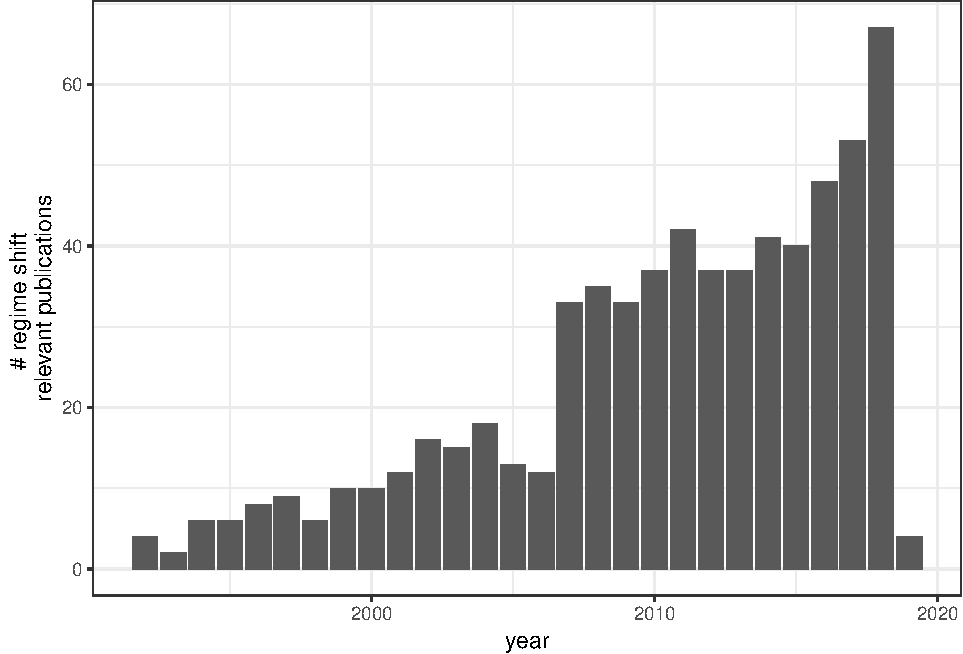
\includegraphics{_myDissertation_files/figure-latex/wosRegimePubsByYear-1.pdf}
\caption{\label{fig:wosRegimePubsByYear}Number of publications by year in
fields `Ecology' and `Biodiversity Conservation' which included terms
related to `regime shift' (total = 654).}
\end{figure}
\section{Results}\label{results}
\begin{figure}
\centering
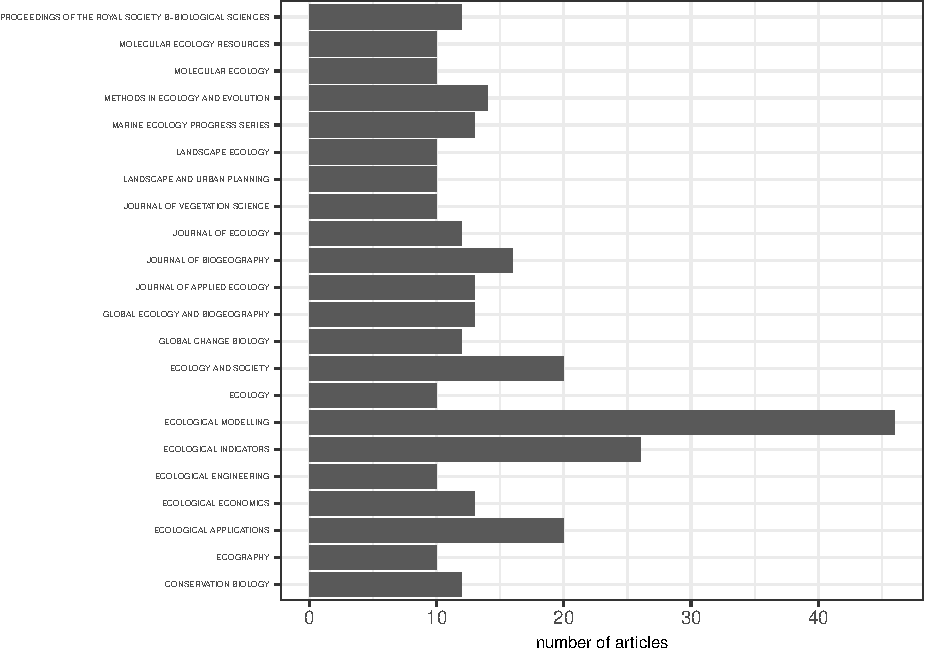
\includegraphics{_myDissertation_files/figure-latex/wosRegimePubsByJrnlmin10Pubs-1.pdf}
\caption{\label{fig:wosRegimePubsByJrnlmin10Pubs}Distribution of the `regime
shift' articles for journals with at least 10 articles.}
\end{figure}
\subsection{Web of Science}\label{web-of-science-1}

The search boolean for WoS boolean \emph{not} including restriction to
fields (WC) `Ecology' and `Conservation Biology' yielded over 20,000
results. Restricting to the abovementioned fields created a manageable
database from which to filter. This search yielded 2,776 articles. 654
of these papers included terms relating to `regime shifts' (Figure
\ref{fig:wosRegimePubsByYear}), many appearing in the journal
\emph{Ecological Modelling} (Figure
\ref{fig:wosRegimePubsByJrnlmin10Pubs}). The rate of publication of
`regime shift' articles is not strongly correlated with the rate of
papers published in `Ecology' and `Biodiversity Conservation' fields
(Figure \ref{fig:wosRegimePubsByYearwithNumEcolPubs}).
\begin{figure}
\centering
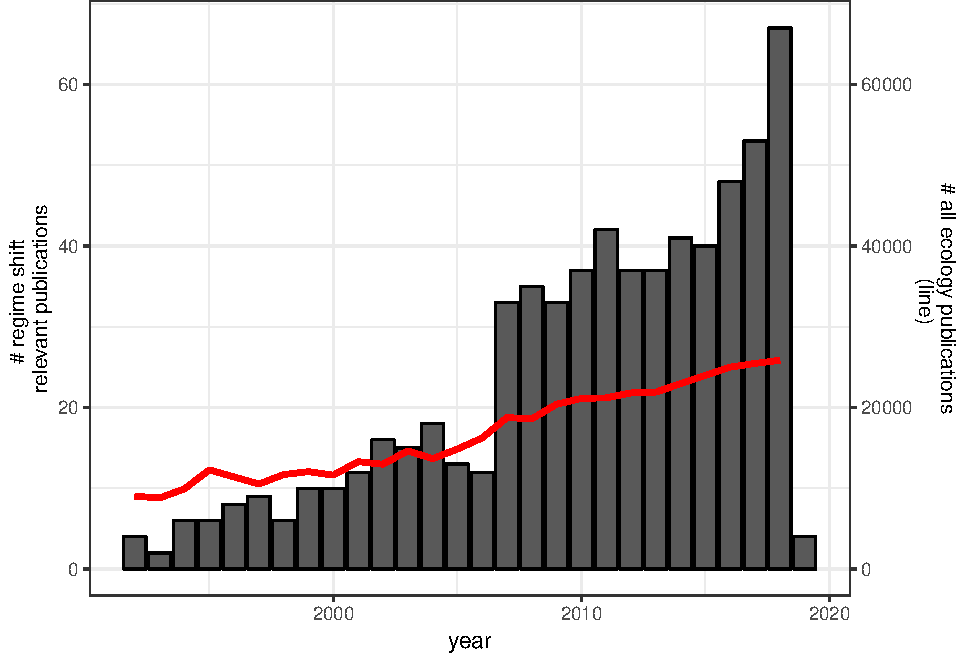
\includegraphics{_myDissertation_files/figure-latex/wosRegimePubsByYearwithNumEcolPubs-1.pdf}
\caption{\label{fig:wosRegimePubsByYearwithNumEcolPubs}Number of
publications by year in fields `Ecology' and `Biodiversity Conservation'
which included terms related to `regime shift' (total = 654).}
\end{figure}
Filtering this WoS results to include only articles mentioning terms
related to `new method' yielded 202 articles. After removing prior
knowledge, only 93 articles remained to be reviewed `by hand' (i.e.,
reading the entire paper). Only 2 `new' methods were identified from the
WoS search (\ref{fig:rdmReviewFlow}).

\subsection{Google Scholar and prior
knowledge}\label{google-scholar-and-prior-knowledge}

Of the 250 articles scanned in Google Scholar, I retained 3 methods. I
was previously aware of an additional 68 articles containing `new'
methods (\ref{fig:rdmReviewFlow}).
\begin{figure}
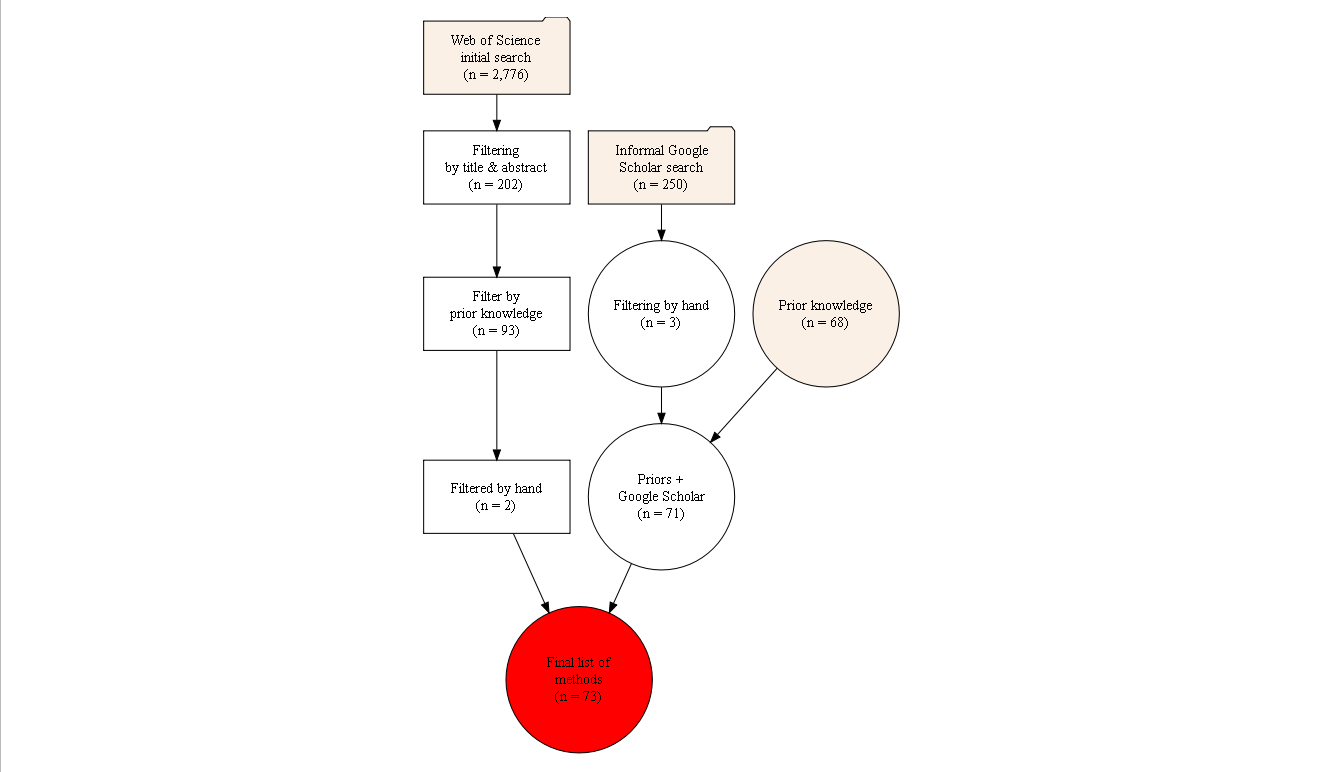
\includegraphics[width=0.95\linewidth]{./chapterFiles/rdmReview/figures/figsCalledInDiss/myDiagraph} \caption{Flowchart of the litearture review process for identifying new regime detection methods. *Only the first ten pages (250 articles) of Google Scholar results were examined. Node shapes: folder = unfiltered articles; box = articles actively filtered; diamond = number of articles with new methods.}\label{fig:rdmReviewFlow}
\end{figure}
\subsection{Regime detection methods identified in
review}\label{regime-detection-methods-identified-in-review}
\begin{longtable}[]{@{}lc@{}}
\caption{List of the regime detection methods identified in this review.
(continued below)}\tabularnewline
\toprule
\begin{minipage}[b]{0.31\columnwidth}\raggedright\strut
Method\strut
\end{minipage} & \begin{minipage}[b]{0.34\columnwidth}\centering\strut
Metric type\strut
\end{minipage}\tabularnewline
\midrule
\endfirsthead
\toprule
\begin{minipage}[b]{0.31\columnwidth}\raggedright\strut
Method\strut
\end{minipage} & \begin{minipage}[b]{0.34\columnwidth}\centering\strut
Metric type\strut
\end{minipage}\tabularnewline
\midrule
\endhead
\begin{minipage}[t]{0.31\columnwidth}\raggedright\strut
Characteristic length scale (CLS) estimation\strut
\end{minipage} & \begin{minipage}[t]{0.34\columnwidth}\centering\strut
attractor reconstruction\strut
\end{minipage}\tabularnewline
\begin{minipage}[t]{0.31\columnwidth}\raggedright\strut
Autocorrelation at-lag-1\strut
\end{minipage} & \begin{minipage}[t]{0.34\columnwidth}\centering\strut
metric\strut
\end{minipage}\tabularnewline
\begin{minipage}[t]{0.31\columnwidth}\raggedright\strut
Autoregressive coefficient of AR(1)\strut
\end{minipage} & \begin{minipage}[t]{0.34\columnwidth}\centering\strut
metric\strut
\end{minipage}\tabularnewline
\begin{minipage}[t]{0.31\columnwidth}\raggedright\strut
Average standard deviates\strut
\end{minipage} & \begin{minipage}[t]{0.34\columnwidth}\centering\strut
metric\strut
\end{minipage}\tabularnewline
\begin{minipage}[t]{0.31\columnwidth}\raggedright\strut
BDS test\strut
\end{minipage} & \begin{minipage}[t]{0.34\columnwidth}\centering\strut
metric\strut
\end{minipage}\tabularnewline
\begin{minipage}[t]{0.31\columnwidth}\raggedright\strut
Coefficient of variation (CV)\strut
\end{minipage} & \begin{minipage}[t]{0.34\columnwidth}\centering\strut
metric\strut
\end{minipage}\tabularnewline
\begin{minipage}[t]{0.31\columnwidth}\raggedright\strut
Conditional heteroskedasticity\strut
\end{minipage} & \begin{minipage}[t]{0.34\columnwidth}\centering\strut
metric\strut
\end{minipage}\tabularnewline
\begin{minipage}[t]{0.31\columnwidth}\raggedright\strut
Cumulative deviation test (CUSUM)\strut
\end{minipage} & \begin{minipage}[t]{0.34\columnwidth}\centering\strut
metric\strut
\end{minipage}\tabularnewline
\begin{minipage}[t]{0.31\columnwidth}\raggedright\strut
Detrended fluctuation analysis\strut
\end{minipage} & \begin{minipage}[t]{0.34\columnwidth}\centering\strut
metric\strut
\end{minipage}\tabularnewline
\begin{minipage}[t]{0.31\columnwidth}\raggedright\strut
Downton-Katz test\strut
\end{minipage} & \begin{minipage}[t]{0.34\columnwidth}\centering\strut
metric\strut
\end{minipage}\tabularnewline
\begin{minipage}[t]{0.31\columnwidth}\raggedright\strut
Fisher Information\strut
\end{minipage} & \begin{minipage}[t]{0.34\columnwidth}\centering\strut
metric\strut
\end{minipage}\tabularnewline
\begin{minipage}[t]{0.31\columnwidth}\raggedright\strut
Intervention Analysis\strut
\end{minipage} & \begin{minipage}[t]{0.34\columnwidth}\centering\strut
metric\strut
\end{minipage}\tabularnewline
\begin{minipage}[t]{0.31\columnwidth}\raggedright\strut
Inverse of AR(1) coefficient\strut
\end{minipage} & \begin{minipage}[t]{0.34\columnwidth}\centering\strut
metric\strut
\end{minipage}\tabularnewline
\begin{minipage}[t]{0.31\columnwidth}\raggedright\strut
Kurtosis\strut
\end{minipage} & \begin{minipage}[t]{0.34\columnwidth}\centering\strut
metric\strut
\end{minipage}\tabularnewline
\begin{minipage}[t]{0.31\columnwidth}\raggedright\strut
LePage test\strut
\end{minipage} & \begin{minipage}[t]{0.34\columnwidth}\centering\strut
metric\strut
\end{minipage}\tabularnewline
\begin{minipage}[t]{0.31\columnwidth}\raggedright\strut
Mann-Kendall test\strut
\end{minipage} & \begin{minipage}[t]{0.34\columnwidth}\centering\strut
metric\strut
\end{minipage}\tabularnewline
\begin{minipage}[t]{0.31\columnwidth}\raggedright\strut
Mann-whitney U-test\strut
\end{minipage} & \begin{minipage}[t]{0.34\columnwidth}\centering\strut
metric\strut
\end{minipage}\tabularnewline
\begin{minipage}[t]{0.31\columnwidth}\raggedright\strut
Moving detrended fluctuation analysis (MDFA)\strut
\end{minipage} & \begin{minipage}[t]{0.34\columnwidth}\centering\strut
metric\strut
\end{minipage}\tabularnewline
\begin{minipage}[t]{0.31\columnwidth}\raggedright\strut
Nearest-neighbor statistics\strut
\end{minipage} & \begin{minipage}[t]{0.34\columnwidth}\centering\strut
metric\strut
\end{minipage}\tabularnewline
\begin{minipage}[t]{0.31\columnwidth}\raggedright\strut
Nikiforiv method\strut
\end{minipage} & \begin{minipage}[t]{0.34\columnwidth}\centering\strut
metric\strut
\end{minipage}\tabularnewline
\begin{minipage}[t]{0.31\columnwidth}\raggedright\strut
Oerleman's method\strut
\end{minipage} & \begin{minipage}[t]{0.34\columnwidth}\centering\strut
metric\strut
\end{minipage}\tabularnewline
\begin{minipage}[t]{0.31\columnwidth}\raggedright\strut
Pettitt test\strut
\end{minipage} & \begin{minipage}[t]{0.34\columnwidth}\centering\strut
metric\strut
\end{minipage}\tabularnewline
\begin{minipage}[t]{0.31\columnwidth}\raggedright\strut
Probability density function entropy method\strut
\end{minipage} & \begin{minipage}[t]{0.34\columnwidth}\centering\strut
metric\strut
\end{minipage}\tabularnewline
\begin{minipage}[t]{0.31\columnwidth}\raggedright\strut
Quickest detection method (ShiryaevRoberts statistic)\strut
\end{minipage} & \begin{minipage}[t]{0.34\columnwidth}\centering\strut
metric\strut
\end{minipage}\tabularnewline
\begin{minipage}[t]{0.31\columnwidth}\raggedright\strut
Rodionov method\strut
\end{minipage} & \begin{minipage}[t]{0.34\columnwidth}\centering\strut
metric\strut
\end{minipage}\tabularnewline
\begin{minipage}[t]{0.31\columnwidth}\raggedright\strut
STARS\strut
\end{minipage} & \begin{minipage}[t]{0.34\columnwidth}\centering\strut
metric\strut
\end{minipage}\tabularnewline
\begin{minipage}[t]{0.31\columnwidth}\raggedright\strut
Sequential tests/moving windows\strut
\end{minipage} & \begin{minipage}[t]{0.34\columnwidth}\centering\strut
metric\strut
\end{minipage}\tabularnewline
\begin{minipage}[t]{0.31\columnwidth}\raggedright\strut
Signal-to-noise ratio\strut
\end{minipage} & \begin{minipage}[t]{0.34\columnwidth}\centering\strut
metric\strut
\end{minipage}\tabularnewline
\begin{minipage}[t]{0.31\columnwidth}\raggedright\strut
Skewness\strut
\end{minipage} & \begin{minipage}[t]{0.34\columnwidth}\centering\strut
metric\strut
\end{minipage}\tabularnewline
\begin{minipage}[t]{0.31\columnwidth}\raggedright\strut
Spectral density\strut
\end{minipage} & \begin{minipage}[t]{0.34\columnwidth}\centering\strut
metric\strut
\end{minipage}\tabularnewline
\begin{minipage}[t]{0.31\columnwidth}\raggedright\strut
Spectral exponent\strut
\end{minipage} & \begin{minipage}[t]{0.34\columnwidth}\centering\strut
metric\strut
\end{minipage}\tabularnewline
\begin{minipage}[t]{0.31\columnwidth}\raggedright\strut
Spectral ratio\strut
\end{minipage} & \begin{minipage}[t]{0.34\columnwidth}\centering\strut
metric\strut
\end{minipage}\tabularnewline
\begin{minipage}[t]{0.31\columnwidth}\raggedright\strut
Spectrum indicator\strut
\end{minipage} & \begin{minipage}[t]{0.34\columnwidth}\centering\strut
metric\strut
\end{minipage}\tabularnewline
\begin{minipage}[t]{0.31\columnwidth}\raggedright\strut
Stability Index of the Ecological Units\strut
\end{minipage} & \begin{minipage}[t]{0.34\columnwidth}\centering\strut
metric\strut
\end{minipage}\tabularnewline
\begin{minipage}[t]{0.31\columnwidth}\raggedright\strut
Standard deviation\strut
\end{minipage} & \begin{minipage}[t]{0.34\columnwidth}\centering\strut
metric\strut
\end{minipage}\tabularnewline
\begin{minipage}[t]{0.31\columnwidth}\raggedright\strut
Standard normal homoegeneity\strut
\end{minipage} & \begin{minipage}[t]{0.34\columnwidth}\centering\strut
metric\strut
\end{minipage}\tabularnewline
\begin{minipage}[t]{0.31\columnwidth}\raggedright\strut
T-test\strut
\end{minipage} & \begin{minipage}[t]{0.34\columnwidth}\centering\strut
metric\strut
\end{minipage}\tabularnewline
\begin{minipage}[t]{0.31\columnwidth}\raggedright\strut
Threshold Indicator Taxa ANalysis (TITAN)\strut
\end{minipage} & \begin{minipage}[t]{0.34\columnwidth}\centering\strut
metric\strut
\end{minipage}\tabularnewline
\begin{minipage}[t]{0.31\columnwidth}\raggedright\strut
Variance Index\strut
\end{minipage} & \begin{minipage}[t]{0.34\columnwidth}\centering\strut
metric\strut
\end{minipage}\tabularnewline
\begin{minipage}[t]{0.31\columnwidth}\raggedright\strut
Wilcoxon rank-sum\strut
\end{minipage} & \begin{minipage}[t]{0.34\columnwidth}\centering\strut
metric\strut
\end{minipage}\tabularnewline
\begin{minipage}[t]{0.31\columnwidth}\raggedright\strut
dimension reduction techniques (e.g., PCA)\strut
\end{minipage} & \begin{minipage}[t]{0.34\columnwidth}\centering\strut
metric\strut
\end{minipage}\tabularnewline
\begin{minipage}[t]{0.31\columnwidth}\raggedright\strut
two-phase regression\strut
\end{minipage} & \begin{minipage}[t]{0.34\columnwidth}\centering\strut
metric of a model\strut
\end{minipage}\tabularnewline
\begin{minipage}[t]{0.31\columnwidth}\raggedright\strut
Zonal thresholding\strut
\end{minipage} & \begin{minipage}[t]{0.34\columnwidth}\centering\strut
metric*\strut
\end{minipage}\tabularnewline
\begin{minipage}[t]{0.31\columnwidth}\raggedright\strut
Bayesian approaches\strut
\end{minipage} & \begin{minipage}[t]{0.34\columnwidth}\centering\strut
model\strut
\end{minipage}\tabularnewline
\begin{minipage}[t]{0.31\columnwidth}\raggedright\strut
Convex model\strut
\end{minipage} & \begin{minipage}[t]{0.34\columnwidth}\centering\strut
model\strut
\end{minipage}\tabularnewline
\begin{minipage}[t]{0.31\columnwidth}\raggedright\strut
Generalized model\strut
\end{minipage} & \begin{minipage}[t]{0.34\columnwidth}\centering\strut
model\strut
\end{minipage}\tabularnewline
\begin{minipage}[t]{0.31\columnwidth}\raggedright\strut
Nonparametric drift-diffusion-jump model\strut
\end{minipage} & \begin{minipage}[t]{0.34\columnwidth}\centering\strut
model\strut
\end{minipage}\tabularnewline
\begin{minipage}[t]{0.31\columnwidth}\raggedright\strut
Potential analysis\strut
\end{minipage} & \begin{minipage}[t]{0.34\columnwidth}\centering\strut
model\strut
\end{minipage}\tabularnewline
\begin{minipage}[t]{0.31\columnwidth}\raggedright\strut
Regression-based models\strut
\end{minipage} & \begin{minipage}[t]{0.34\columnwidth}\centering\strut
model\strut
\end{minipage}\tabularnewline
\begin{minipage}[t]{0.31\columnwidth}\raggedright\strut
Self-exciting threshold autoregressive state-space model
SETARSS(p)\strut
\end{minipage} & \begin{minipage}[t]{0.34\columnwidth}\centering\strut
model\strut
\end{minipage}\tabularnewline
\begin{minipage}[t]{0.31\columnwidth}\raggedright\strut
Smooth transition autoregressive model\strut
\end{minipage} & \begin{minipage}[t]{0.34\columnwidth}\centering\strut
model\strut
\end{minipage}\tabularnewline
\begin{minipage}[t]{0.31\columnwidth}\raggedright\strut
Time-varying AR(p) model\strut
\end{minipage} & \begin{minipage}[t]{0.34\columnwidth}\centering\strut
model\strut
\end{minipage}\tabularnewline
\begin{minipage}[t]{0.31\columnwidth}\raggedright\strut
shiftogram\strut
\end{minipage} & \begin{minipage}[t]{0.34\columnwidth}\centering\strut
model\strut
\end{minipage}\tabularnewline
\begin{minipage}[t]{0.31\columnwidth}\raggedright\strut
Online dynamic linear modelling + time\_varying autoregressive
state\_space models (TVARSS)\strut
\end{minipage} & \begin{minipage}[t]{0.34\columnwidth}\centering\strut
models\strut
\end{minipage}\tabularnewline
\begin{minipage}[t]{0.31\columnwidth}\raggedright\strut
Clustering, various\strut
\end{minipage} & \begin{minipage}[t]{0.34\columnwidth}\centering\strut
NA\strut
\end{minipage}\tabularnewline
\begin{minipage}[t]{0.31\columnwidth}\raggedright\strut
Fourier Analysis\strut
\end{minipage} & \begin{minipage}[t]{0.34\columnwidth}\centering\strut
NA\strut
\end{minipage}\tabularnewline
\begin{minipage}[t]{0.31\columnwidth}\raggedright\strut
Free-knot splines \& piecewise linear modelling\strut
\end{minipage} & \begin{minipage}[t]{0.34\columnwidth}\centering\strut
NA\strut
\end{minipage}\tabularnewline
\begin{minipage}[t]{0.31\columnwidth}\raggedright\strut
Lanzante method\strut
\end{minipage} & \begin{minipage}[t]{0.34\columnwidth}\centering\strut
NA\strut
\end{minipage}\tabularnewline
\begin{minipage}[t]{0.31\columnwidth}\raggedright\strut
MCMC\strut
\end{minipage} & \begin{minipage}[t]{0.34\columnwidth}\centering\strut
NA\strut
\end{minipage}\tabularnewline
\begin{minipage}[t]{0.31\columnwidth}\raggedright\strut
Method 1-TBD\strut
\end{minipage} & \begin{minipage}[t]{0.34\columnwidth}\centering\strut
NA\strut
\end{minipage}\tabularnewline
\begin{minipage}[t]{0.31\columnwidth}\raggedright\strut
Method 2-TBD\strut
\end{minipage} & \begin{minipage}[t]{0.34\columnwidth}\centering\strut
NA\strut
\end{minipage}\tabularnewline
\begin{minipage}[t]{0.31\columnwidth}\raggedright\strut
Vector-autoregressive method\strut
\end{minipage} & \begin{minipage}[t]{0.34\columnwidth}\centering\strut
NA\strut
\end{minipage}\tabularnewline
\begin{minipage}[t]{0.31\columnwidth}\raggedright\strut
Wavelet analysis (decomposition)\strut
\end{minipage} & \begin{minipage}[t]{0.34\columnwidth}\centering\strut
NA\strut
\end{minipage}\tabularnewline
\begin{minipage}[t]{0.31\columnwidth}\raggedright\strut
method-fuzzy synthetic evaluation (FSE)\strut
\end{minipage} & \begin{minipage}[t]{0.34\columnwidth}\centering\strut
NA\strut
\end{minipage}\tabularnewline
\bottomrule
\end{longtable}
\begin{longtable}[]{@{}c@{}}
\toprule
\begin{minipage}[b]{0.44\columnwidth}\centering\strut
Source\strut
\end{minipage}\tabularnewline
\midrule
\endhead
\begin{minipage}[t]{0.44\columnwidth}\centering\strut
@NA\strut
\end{minipage}\tabularnewline
\begin{minipage}[t]{0.44\columnwidth}\centering\strut
@vincent1998technique\strut
\end{minipage}\tabularnewline
\begin{minipage}[t]{0.44\columnwidth}\centering\strut
@held2004detection\strut
\end{minipage}\tabularnewline
\begin{minipage}[t]{0.44\columnwidth}\centering\strut
@ebbesmeyer19911976\strut
\end{minipage}\tabularnewline
\begin{minipage}[t]{0.44\columnwidth}\centering\strut
@carpenterBrock2011early\strut
\end{minipage}\tabularnewline
\begin{minipage}[t]{0.44\columnwidth}\centering\strut
@carpenter2006rising\strut
\end{minipage}\tabularnewline
\begin{minipage}[t]{0.44\columnwidth}\centering\strut
@seekell2011conditional\strut
\end{minipage}\tabularnewline
\begin{minipage}[t]{0.44\columnwidth}\centering\strut
@buishand1982some\strut
\end{minipage}\tabularnewline
\begin{minipage}[t]{0.44\columnwidth}\centering\strut
@livina2007modified\strut
\end{minipage}\tabularnewline
\begin{minipage}[t]{0.44\columnwidth}\centering\strut
@karl1987approach\strut
\end{minipage}\tabularnewline
\begin{minipage}[t]{0.44\columnwidth}\centering\strut
@fath\_regime\_2003\strut
\end{minipage}\tabularnewline
\begin{minipage}[t]{0.44\columnwidth}\centering\strut
@francis1994decadal\strut
\end{minipage}\tabularnewline
\begin{minipage}[t]{0.44\columnwidth}\centering\strut
@carpenter2008leading\strut
\end{minipage}\tabularnewline
\begin{minipage}[t]{0.44\columnwidth}\centering\strut
@biggs2009turning\strut
\end{minipage}\tabularnewline
\begin{minipage}[t]{0.44\columnwidth}\centering\strut
@yonetani1993detection\strut
\end{minipage}\tabularnewline
\begin{minipage}[t]{0.44\columnwidth}\centering\strut
@goossens1987recognize\strut
\end{minipage}\tabularnewline
\begin{minipage}[t]{0.44\columnwidth}\centering\strut
@mauget2003multidecadal\strut
\end{minipage}\tabularnewline
\begin{minipage}[t]{0.44\columnwidth}\centering\strut
@he2008new\strut
\end{minipage}\tabularnewline
\begin{minipage}[t]{0.44\columnwidth}\centering\strut
@pawlowski\_identification\_2008\strut
\end{minipage}\tabularnewline
\begin{minipage}[t]{0.44\columnwidth}\centering\strut
@NA\strut
\end{minipage}\tabularnewline
\begin{minipage}[t]{0.44\columnwidth}\centering\strut
@oerlemans1978objective\strut
\end{minipage}\tabularnewline
\begin{minipage}[t]{0.44\columnwidth}\centering\strut
@pettitt1979non\strut
\end{minipage}\tabularnewline
\begin{minipage}[t]{0.44\columnwidth}\centering\strut
@pawlowski\_identification\_2008\strut
\end{minipage}\tabularnewline
\begin{minipage}[t]{0.44\columnwidth}\centering\strut
@moustakides2009numerical\strut
\end{minipage}\tabularnewline
\begin{minipage}[t]{0.44\columnwidth}\centering\strut
@rodionov\_sequential\_2005\strut
\end{minipage}\tabularnewline
\begin{minipage}[t]{0.44\columnwidth}\centering\strut
@buishand1982some\strut
\end{minipage}\tabularnewline
\begin{minipage}[t]{0.44\columnwidth}\centering\strut
@NA\strut
\end{minipage}\tabularnewline
\begin{minipage}[t]{0.44\columnwidth}\centering\strut
@NA\strut
\end{minipage}\tabularnewline
\begin{minipage}[t]{0.44\columnwidth}\centering\strut
@guttal2008changing\strut
\end{minipage}\tabularnewline
\begin{minipage}[t]{0.44\columnwidth}\centering\strut
@kleinen2003potential\strut
\end{minipage}\tabularnewline
\begin{minipage}[t]{0.44\columnwidth}\centering\strut
@andersen\_ecological\_2009\strut
\end{minipage}\tabularnewline
\begin{minipage}[t]{0.44\columnwidth}\centering\strut
@biggs2009turning\strut
\end{minipage}\tabularnewline
\begin{minipage}[t]{0.44\columnwidth}\centering\strut
@NA\strut
\end{minipage}\tabularnewline
\begin{minipage}[t]{0.44\columnwidth}\centering\strut
@parparov2015quantifying\strut
\end{minipage}\tabularnewline
\begin{minipage}[t]{0.44\columnwidth}\centering\strut
@carpenter2006rising\strut
\end{minipage}\tabularnewline
\begin{minipage}[t]{0.44\columnwidth}\centering\strut
@alexandersson1986homogeneity\strut
\end{minipage}\tabularnewline
\begin{minipage}[t]{0.44\columnwidth}\centering\strut
@ducre2003comparison\strut
\end{minipage}\tabularnewline
\begin{minipage}[t]{0.44\columnwidth}\centering\strut
@baker2010new\strut
\end{minipage}\tabularnewline
\begin{minipage}[t]{0.44\columnwidth}\centering\strut
@brock\_variance\_2006\strut
\end{minipage}\tabularnewline
\begin{minipage}[t]{0.44\columnwidth}\centering\strut
@karl1987approach\strut
\end{minipage}\tabularnewline
\begin{minipage}[t]{0.44\columnwidth}\centering\strut
@NA\strut
\end{minipage}\tabularnewline
\begin{minipage}[t]{0.44\columnwidth}\centering\strut
@easterling1995new\strut
\end{minipage}\tabularnewline
\begin{minipage}[t]{0.44\columnwidth}\centering\strut
@yin2017methods\strut
\end{minipage}\tabularnewline
\begin{minipage}[t]{0.44\columnwidth}\centering\strut
@jo2016bayesian\strut
\end{minipage}\tabularnewline
\begin{minipage}[t]{0.44\columnwidth}\centering\strut
@qi2016resilience\strut
\end{minipage}\tabularnewline
\begin{minipage}[t]{0.44\columnwidth}\centering\strut
@lade2012early\strut
\end{minipage}\tabularnewline
\begin{minipage}[t]{0.44\columnwidth}\centering\strut
@carpenter2011early\strut
\end{minipage}\tabularnewline
\begin{minipage}[t]{0.44\columnwidth}\centering\strut
@ives2012detecting\strut
\end{minipage}\tabularnewline
\begin{minipage}[t]{0.44\columnwidth}\centering\strut
@solow1987testing\strut
\end{minipage}\tabularnewline
\begin{minipage}[t]{0.44\columnwidth}\centering\strut
@tong1990nonlinear\strut
\end{minipage}\tabularnewline
\begin{minipage}[t]{0.44\columnwidth}\centering\strut
@see gal2010novel\strut
\end{minipage}\tabularnewline
\begin{minipage}[t]{0.44\columnwidth}\centering\strut
@ives2012detecting\strut
\end{minipage}\tabularnewline
\begin{minipage}[t]{0.44\columnwidth}\centering\strut
@groger2011analyses\strut
\end{minipage}\tabularnewline
\begin{minipage}[t]{0.44\columnwidth}\centering\strut
@parparov2017quantifying\strut
\end{minipage}\tabularnewline
\begin{minipage}[t]{0.44\columnwidth}\centering\strut
@NA\strut
\end{minipage}\tabularnewline
\begin{minipage}[t]{0.44\columnwidth}\centering\strut
@carpenter2010early\strut
\end{minipage}\tabularnewline
\begin{minipage}[t]{0.44\columnwidth}\centering\strut
@gal2010novel\strut
\end{minipage}\tabularnewline
\begin{minipage}[t]{0.44\columnwidth}\centering\strut
@lanzante1996resistant\strut
\end{minipage}\tabularnewline
\begin{minipage}[t]{0.44\columnwidth}\centering\strut
@NA\strut
\end{minipage}\tabularnewline
\begin{minipage}[t]{0.44\columnwidth}\centering\strut
@manly2006two\strut
\end{minipage}\tabularnewline
\begin{minipage}[t]{0.44\columnwidth}\centering\strut
@manly2006two\strut
\end{minipage}\tabularnewline
\begin{minipage}[t]{0.44\columnwidth}\centering\strut
@solow\_test\_2005\strut
\end{minipage}\tabularnewline
\begin{minipage}[t]{0.44\columnwidth}\centering\strut
@cazelles2008wavelet\strut
\end{minipage}\tabularnewline
\begin{minipage}[t]{0.44\columnwidth}\centering\strut
@wang2011application\strut
\end{minipage}\tabularnewline
\bottomrule
\end{longtable}
Using my prior knowledge of the relevant litearture, referring to
previous review articles, and searching both Web of Science and Google
Scholar, I identified 64 unique regime detection measures (Figure
\ref{fig:rdmReviewFlow}; Table \ref{tab:methodsMetricsListTab1}).
\begin{figure}
\centering
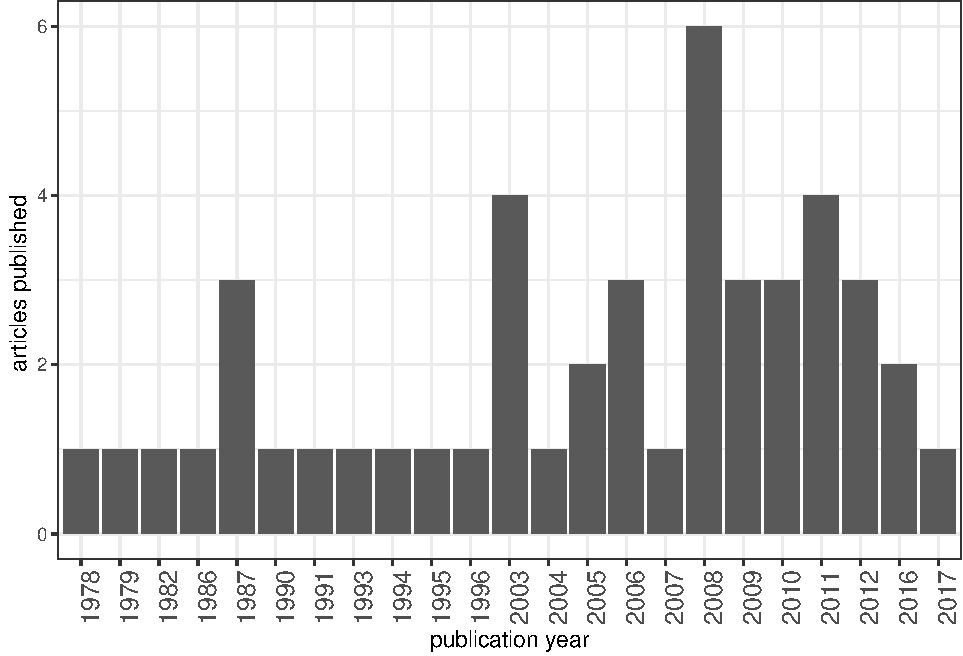
\includegraphics{_myDissertation_files/figure-latex/jrnlYearFig-1.pdf}
\caption{\label{fig:jrnlYearFig}Number of methods publisheed over time.}
\end{figure}
\section{Discussion}\label{discussion}

In this chapter I highlighted the plethora of regime detection metrics
proposed in the literature for analyzing ecological data (Table
\ref{tab:methodsMetricsListTab1}). Although multiple reviews of regime
detection measures exist, they are not comprehensive in their survey of
the possible methods. Most reviews have summarized various aspects of
regime detection measures. For example, Roberts et al. (2018) summarizes
methods capable of handling multiple (c.f. a single) variable, and Dakos
et al. (2015b) review only methods designed to detect the phenomenon of
critical slowing down. Here, I did not discriminate--rather, I present
an exaustive list of the plethora of methods proposed for detecting
ecological detect regime shifts, \emph{sensu lato}, providing a
much-needed update to collection provided by Rodionov (2005), and other
review papers (Mac Nally et al., 2014, Scheffer et al. (2015), Rodionov
(2005), Roberts et al. (2018), Dakos et al. (2015b), Mantua (2004),
Litzow \& Hunsicker (2016), Kefi et al. (2014), Andersen et al. (2009),
Boettiger et al. (2013), Dakos et al. (2015a), Clements \& Ozgul (2018),
Filatova et al. (2016), deYoung et al. (2008)).

\subsection{Barriers to identifying new regime detection
measures}\label{barriers-to-identifying-new-regime-detection-measures}

Clearly, as was shown in this chapter (Figure \ref{fig:rdmReviewFlow}),
a systematic review of the ecological literature will likely not yield
anywhere near a comprehensive list of the regime detection measures
proposed and/or used. This disaparity may be due to both my search
methods and to the current state of regime shift research in ecology.

First, my review restricted articles to articles suggesting they were
introducing a `new method' as n RDM. Avoiding this potential barrier
would have required I review the titles, abstracts, and bodies of over
22,000 articles (Figure \ref{fig:rdmReviewFlow}). Alternatively, this
may also be ameliorated by searching the relevant literature for
\emph{applications} of regime detection measures to ecological data,
however, I suspect this would similarly yield a large number of articles
to review.

Next, only a handful of methods have been introduced to the mainstream
methodological journals in ecology (e.g., \emph{Ecological Modelling},
\emph{Methods in Ecology and Evolution}; Figure \ref{fig:jrnlDistFig}).
Although many mainstream publications (e.g., \emph{Science},
\emph{Ecology Letters}) include applications of some of the methods
identified in this chapter (Table \ref{tab:methodsMetricsListTab1}), I
argue that celebrity and `new and shiny' (Steel, Kennedy, Cunningham, \&
Stanovick, 2013) methods may influence which methodological articles are
printed in these popular journals.
\begin{figure}
\centering
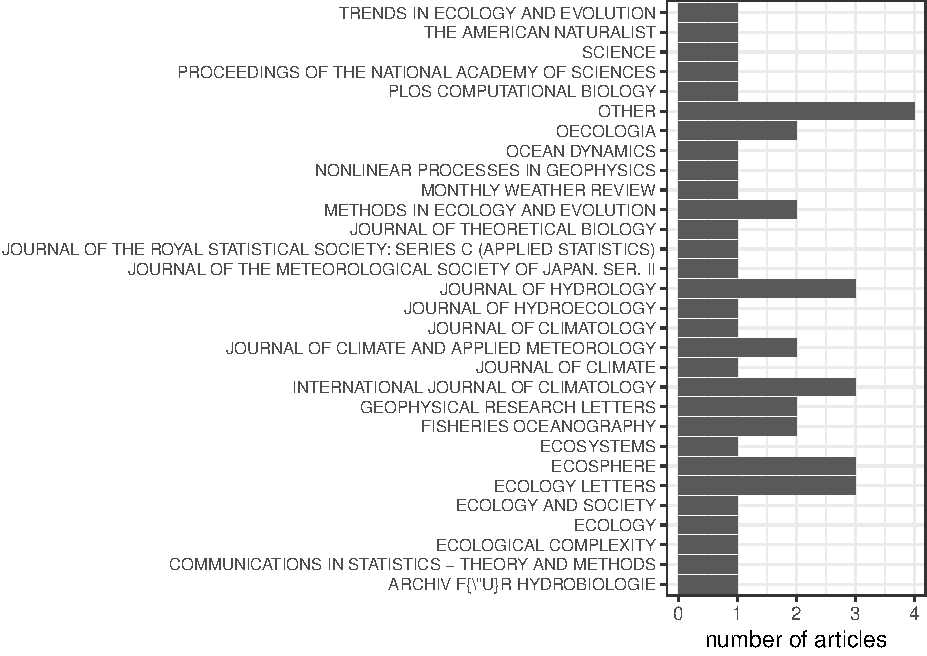
\includegraphics{_myDissertation_files/figure-latex/jrnlDistFig-1.pdf}
\caption{\label{fig:jrnlDistFig}Distribution of identified methods across
publications. Note: books, reports, and articles without original
reference coded as `Other'}
\end{figure}
A critical survey of potetial and realized applications of these methods
would be useful for highlighting the needs of future research and
methodological improvements. Many of the methods presented in Table
\ref{tab:methodsMetricsListTab1} have either not been applied to
empirical data at all, or were tested only once (often but not always in
the article introducing the method). Some methods, especially those
dubbed `early warning indicators' (variance, autoregressive model
coefficients) have become relativley mainstream in their application to
empirical data, however, have been shown to be less robust to noisy and
nonlinear systems data (Burthe et al., 2016) and systems not exhibiting
catstrophic shifts (Dutta, Sharma, \& Abbott, 2018). Most other methods
have yet to be rigorously tested on noisy, high dimensional, empirical
data. Further, the methods which are not mainstream but have been
applied to one of these data types have not any statistical indicators
associated with confirming the existence and location of the regime
shift.

As shown this chapter, identifying regime detection measures using
traditional literature review techniques may prove difficult. Many of
the methods identified in my review were not identified using Web of
Science or Google Scholar--rather, I was either previously aware of most
of the methods, and many others were highlighted in previous RDM
reviews. To facilitate this process, an online, comprehensive database
may prove useful to the practical ecologist.

\subsection{Reducing the barriers to regime detection
measures}\label{reducing-the-barriers-to-regime-detection-measures}

To make the regime detection measures more available and transparent to
the practical ecologist, I recommend the following: 1. consitent use of
fewer methods 1. persistent collection and maintenance of baseline data
(reference data) 1. an on-line database of all methods - open-sourced -
linked to the original sources (in ecology and statistics or
mathematics) - linked to applications 1. a critical review of the
current state of methods in ecology - including methodological
advancements - especially highlighting where the method fails to perform
- including historical tracking of specific methods to identify which
may need to be retired, rather than resuscitated 1. more empirical
applications of these methods (especially of those only tested on toy
and experimental data) 1. relation of RDMs in ecology to other fields
(computer science, data science, climatology and oceanography)

I suggest below a suite of questions which may provide useful in a
critical review of the characteristics, rigor, and promise of methods in
the context of ecological data analysis.
\begin{longtable}{>{\bfseries}l|>{\raggedright\arraybackslash}p{30em}}
\caption{\label{tab:nextStepsTab}Potential questions for a comprehensive review of the ecological regime detection metrics literature.}\\
\toprule
Type & Questions\\
\midrule
Methodological & What are the major assumptions about the distribution?\\
 & Does the method explicitly assume stationarity? If not, can it handle non-stationary processes?\\
 & Does the performance of the method change with non-stationarity?\\
 & Can the method handle unstructured data (information)?\\
 & Does the regime shift need to be identified *a priori*?\\
\addlinespace
 & Can the method handle multiple regime shifts?\\
 & Does the performance of the method change with non-stationarity?\\
 & What types of regime shifts can the method detect (e.g., stochastic resonance, slow-fast cycles, noise-induced transition)?\\
 & Is it a model- or metric-based method?\\
 & Does it have forecasting potential?\\
\addlinespace
 & Can the method handle uneven sampling?\\
 & What are the minimum data requirements (resolution, extent, number of observations)?\\
 & How does the method handle missing data (e.g., new invasions)?\\
 & Does the method assume Eulerian or Lagrangian processes?\\
Ecological & Has the method been tested on empirical data? If so, to what rigor?\\
\addlinespace
 & What is the impact of losing state variables on long-term predictions (e.g., species extinction)?\\
 & Can the method identify drivers?\\
 & What assumptions does the method make about the system?\\
 & What types of regime shifts are possible in the system?\\
 & Are regime shift(s) suspected *a priori*?\\
\addlinespace
 & What lag(s) exist in the data (system)?\\
 & Would a positive forecast change management action?\\
 & Do predictions translate to other systems?\\
 & Can we interpolate data if necessary? If so, what does this mean for inference?\\
 & In which discipline(s) beyond ecology has the method been tested?\\
\bottomrule
\end{longtable}
\hypertarget{refs}{}
\hypertarget{ref-andersen_ecological_2009}{}
Andersen, T., Carstensen, J., Hern??ndez-Garc??a, E., \& Duarte, C. M.
(2009). Ecological thresholds and regime shifts: Approaches to
identification. \emph{Trends in Ecology \& Evolution}, \emph{24}(1),
49--57. \url{http://doi.org/10.1016/j.tree.2008.07.014}

\hypertarget{ref-boettiger_early_2013}{}
Boettiger, C., Ross, N., \& Hastings, A. (2013). Early warning signals:
The charted and uncharted territories. \emph{Theoretical Ecology},
\emph{6}(3), 255--264.

\hypertarget{ref-burthe2016early}{}
Burthe, S. J., Henrys, P. A., Mackay, E. B., Spears, B. M., Campbell,
R., Carvalho, L., \ldots{} others. (2016). Do early warning indicators
consistently predict nonlinear change in long-term ecological data?
\emph{Journal of Applied Ecology}, \emph{53}(3), 666--676.

\hypertarget{ref-byrski2016double}{}
Byrski, J., \& Byrski, W. (2016). A double window state observer for
detection and isolation of abrupt changes in parameters.
\emph{International Journal of Applied Mathematics and Computer
Science}, \emph{26}(3), 585--602.

\hypertarget{ref-clements2018indicators}{}
Clements, C. F., \& Ozgul, A. (2018). Indicators of transitions in
biological systems. \emph{Ecology Letters}, \emph{21}(6), 905--919.

\hypertarget{ref-dakos_resilience_2015}{}
Dakos, V., Carpenter, S. R., Nes, E. H. van, \& Scheffer, M. (2015a).
Resilience indicators: Prospects and limitations for early warnings of
regime shifts. \emph{Philosophical Transactions of the Royal Society B:
Biological Sciences}, \emph{370}(1659), 20130263.
\url{http://doi.org/10.1098/rstb.2013.0263}

\hypertarget{ref-dakos2015resilience}{}
Dakos, V., Carpenter, S. R., Nes, E. H. van, \& Scheffer, M. (2015b).
Resilience indicators: Prospects and limitations for early warnings of
regime shifts. \emph{Philosophical Transactions of the Royal Society B:
Biological Sciences}, \emph{370}(1659), 20130263.

\hypertarget{ref-davis_comparing_2008}{}
Davis, E. P., \& Karim, D. (2008). Comparing early warning systems for
banking crises. \emph{Journal of Financial Stability}, \emph{4}(2),
89--120.

\hypertarget{ref-deyoung_regime_2008}{}
deYoung, B., Barange, M., Beaugrand, G., Harris, R., Perry, R. I.,
Scheffer, M., \& Werner, F. (2008). Regime shifts in marine ecosystems:
Detection, prediction and management. \emph{Trends in Ecology \&
Evolution}, \emph{23}(7), 402--409.
\url{http://doi.org/10.1016/j.tree.2008.03.008}

\hypertarget{ref-ducre2003comparison}{}
Ducré-Robitaille, J.-F., Vincent, L. A., \& Boulet, G. (2003).
Comparison of techniques for detection of discontinuities in temperature
series. \emph{International Journal of Climatology: A Journal of the
Royal Meteorological Society}, \emph{23}(9), 1087--1101.

\hypertarget{ref-dutta2018robustness}{}
Dutta, P. S., Sharma, Y., \& Abbott, K. C. (2018). Robustness of early
warning signals for catastrophic and non-catastrophic transitions.
\emph{Oikos}, \emph{127}(9), 1251--1263.

\hypertarget{ref-filatova2016regime}{}
Filatova, T., Polhill, J. G., \& Ewijk, S. van. (2016). Regime shifts in
coupled socio-environmental systems: Review of modelling challenges and
approaches. \emph{Environmental Modelling \& Software}, \emph{75},
333--347.

\hypertarget{ref-kefi2014early}{}
Kefi, S., Guttal, V., Brock, W. A., Carpenter, S. R., Ellison, A. M.,
Livina, V. N., \ldots{} Dakos, V. (2014). Early warning signals of
ecological transitions: Methods for spatial patterns. \emph{PloS One},
\emph{9}(3), e92097.

\hypertarget{ref-kong2017hydrological}{}
Kong, X., He, Q., Yang, B., He, W., Xu, F., Janssen, A. B., \ldots{}
others. (2017). Hydrological regulation drives regime shifts: Evidence
from paleolimnology and ecosystem modeling of a large shallow chinese
lake. \emph{Global Change Biology}, \emph{23}(2), 737--754.

\hypertarget{ref-litzow_early_2016}{}
Litzow, M. A., \& Hunsicker, M. E. (2016). Early warning signals,
nonlinearity, and signs of hysteresis in real ecosystems.
\emph{Ecosphere}, \emph{7}(12), n/a--n/a.
\url{http://doi.org/10.1002/ecs2.1614}

\hypertarget{ref-liu_complexity_2007}{}
Liu, J., Dietz, T., Carpenter, S. R., Alberti, M., Folke, C., Moran, E.,
\ldots{} others. (2007). Complexity of coupled human and natural
systems. \emph{Science}, \emph{317}(5844), 1513--1516.

\hypertarget{ref-mac2014scrutiny}{}
Mac Nally, R., Albano, C., \& Fleishman, E. (2014). A scrutiny of the
evidence for pressure-induced state shifts in estuarine and nearshore
ecosystems. \emph{Austral Ecology}, \emph{39}(8), 898--906.

\hypertarget{ref-mantua_methods_2004}{}
Mantua, N. (2004). Methods for detecting regime shifts in large marine
ecosystems: A review with approaches applied to North Pacific data.
\emph{Progress in Oceanography}, \emph{60}(2), 165--182.
\url{http://doi.org/10.1016/j.pocean.2004.02.016}

\hypertarget{ref-nicholls_detection_2011}{}
Nicholls, K. H. (2011). Detection of regime shifts in multi-species
communities: The Bay of Quinte phytoplankton example. \emph{Methods in
Ecology and Evolution}, \emph{2}(4), 416--426.
\url{http://doi.org/10.1111/j.2041-210X.2011.00093.x}

\hypertarget{ref-nicholls2011biological}{}
Nicholls, K., Hoyle, J., Johannsson, O., \& Dermott, R. (2011). A
biological regime shift in the bay of quinte ecosystem (lake ontario)
associated with the establishment of invasive dreissenid mussels.
\emph{Journal of Great Lakes Research}, \emph{37}(2), 310--317.

\hypertarget{ref-roberts2018early}{}
Roberts, C. P., Twidwell, D., Burnett, J. L., Donovan, V. M., Wonkka, C.
L., Bielski, C. L., \ldots{} others. (2018). Early warnings for state
transitions. \emph{Rangeland Ecology \& Management}, \emph{71}(6),
659--670.

\hypertarget{ref-rodionov_brief_2005}{}
Rodionov, S. N. (2005). A brief overview of the regime shift detection
methods. \emph{Large-Scale Disturbances (Regime Shifts) and Recovery in
Aquatic Ecosystems: Challenges for Management Toward Sustainability},
17--24. Retrieved from
\url{http://www.beringclimate.noaa.gov/regimes/rodionov_overview.pdf}

\hypertarget{ref-salehpour2011line}{}
Salehpour, S., Gustafsson, T., \& Johansson, A. (2011). An on-line
method for estimation of piecewise constant parameters in linear
regression models. \emph{IFAC Proceedings Volumes}, \emph{44}(1),
3171--3176.

\hypertarget{ref-scheffer_critical_2009}{}
Scheffer, M. (2009). \emph{Critical transitions in nature and society}.
Princeton University Press.

\hypertarget{ref-scheffer2015generic}{}
Scheffer, M., Carpenter, S. R., Dakos, V., \& Nes, E. H. van. (2015).
Generic indicators of ecological resilience: Inferring the chance of a
critical transition. \emph{Annual Review of Ecology, Evolution, and
Systematics}, \emph{46}, 145--167.

\hypertarget{ref-seddon2014quantitative}{}
Seddon, A. W., Froyd, C. A., Witkowski, A., \& Willis, K. J. (2014). A
quantitative framework for analysis of regime shifts in a galápagos
coastal lagoon. \emph{Ecology}, \emph{95}(11), 3046--3055.

\hypertarget{ref-steel2013applied}{}
Steel, E. A., Kennedy, M. C., Cunningham, P. G., \& Stanovick, J. S.
(2013). Applied statistics in ecology: Common pitfalls and simple
solutions. \emph{Ecosphere}, \emph{4}(9), 1--13.

\hypertarget{ref-vasilakopoulos2017resilience}{}
Vasilakopoulos, P., Raitsos, D. E., Tzanatos, E., \& Maravelias, C. D.
(2017). Resilience and regime shifts in a marine biodiversity hotspot.
\emph{Scientific Reports}, \emph{7}(1), 13647.

\hypertarget{ref-yin2017methods}{}
Yin, D., Leroux, S. J., \& He, F. (2017). Methods and models for
identifying thresholds of habitat loss. \emph{Ecography}, \emph{40}(1),
131--143.

\hypertarget{ref-zhou2008one}{}
Zhou, T., \& Shumway, R. (2008). One-step approximations for detecting
regime changes in the state space model with application to the
influenza data. \emph{Computational Statistics \& Data Analysis},
\emph{52}(5), 2277--2291.


\end{document}
